%------------------------------------------------------------------------------
% setup.tex
%
% This illustrates the student conclusion. 
%------------------------------------------------------------------------------
\addcontentsline{toc}{chapter}{Setup del progetto}
\chapter*{setup del progetto}
\label{setup}
Nel seguente appendice sono descritte le procedure necessarie ad una corretta compilazione ed esecuzione del progetto oggetto della relazione.

\addcontentsline{toc}{section}{Compilazione}
\section*{compilazione}
\label{setup-compile}
La parte costituente il \english{core} del simulatore è stata scritta utilizzando il linguaggio Scala ed è composta da differenti moduli; è perciò necessario avere una installazione funzionante dei seguenti \english{software} al fine di completare correttamente la fase di compilazione e produrre cosi gli eseguibili necessari ad avviare il simulatore:

\begin{itemize}
\item{\ac{jre} (\small{testato su versione 1.8.0\_31});}
\item{\ac{jdk} (\small{testato su versione 1.8.0\_31});}
\item{\ac{sre} (\small{sviluppato su versione 2.11.7});}
\item{\ac{sbt} (\small{sviluppato su versione 0.13.9}).}
\end{itemize}

Al fine di ottenere un progetto in linea con i criteri imposti dall'ingegneria del \english{software}, si è deciso di scomporre il progetto in tre macro moduli. Tale suddivisione ha portato ad un alto grado di riutilizzo del codice, aumentato la testabilità e la manutenibilità dello stesso. I moduli risultanti sono i seguenti:

\begin{itemize}
\item{\english{\keyword{core}}: contiene le componenti comuni agli altri moduli del progetto, definendo ciò che è necessario per poter far operare correttamente il nodo città (\english{master}) ed i nodi distretto (\english{slave}). All'interno sono definiti gli attori che compongono il sistema, gli oggetti di \english{business}, i messaggi scambiati, ecc.;}
\item{\english{\keyword{city}}: contiene il codice necessario ad inizializzare ed avviare il nodo ``città";}
\item{\english{\keyword{district}}: contiene il codice necessario ad inizializzare ed avviare un nodo ``distretto''.}
\end{itemize}

Essi vanno cosi a comporre il \english{filesystem}\footnote{In figura sono riportate solo le parti di interesse del \english{filesystem} del progetto. Eventuali cartelle di lavoro verranno costruite in automatico durante la fase di compilazione.} riportato in Figura \ref{setup-compile-structure}.

E' opportuno osservare l'esistenza di un quarto modulo, denominato ``\english{\keyword{project}}'', esso contiene alcuni istruzioni necessarie al sistema di \english{build} \ac{sbt} per poter eseguire correttamente la fase di \english{build} del progetto.

\begin{figure}[h]
\centering
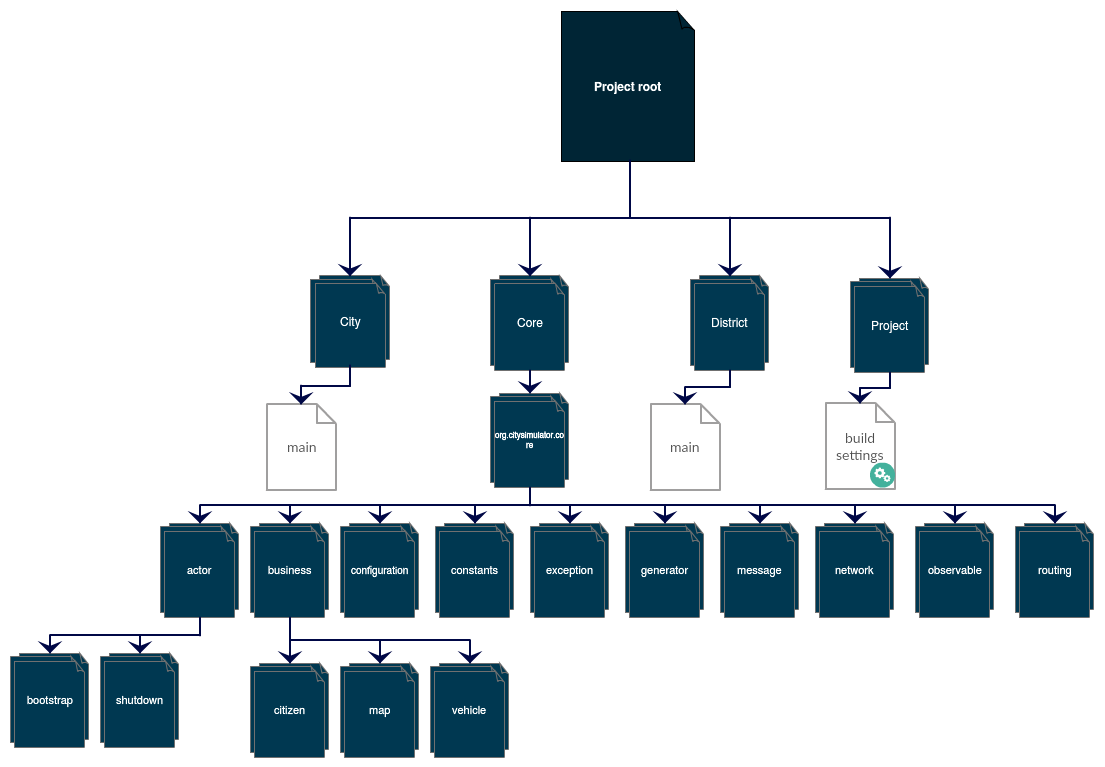
\includegraphics[scale=0.4]{images/configuration/project-design.png}
\caption{\english{Filesystem} contenente il progetto}
\label{setup-compile-structure}
\end{figure}

Per ottenere entrambi gli eseguibili con cui è possibile eseguire il progetto è necessario posizionarsi, via \english{shell}, nella directory \english{root} del progetto ed eseguire il software \ac{sbt} con il comando:

> \textbf{sbt}

Per compilare il modulo rappresentante il nodo centrale, il nodo ``città'', eseguire i seguenti comandi nella \english{shell} \ac{sbt} che si è aperta:

> \textbf{project city}\\
> \textbf{assembly}

Il primo comando sposta l'interprete \ac{sbt} all'interno della sotto-cartella contenente il progetto relativo al nodo ``città'' mentre il secondo esegue la compilazione del modulo e la costruzione di un \acs{jar} con tutte le dipendenze auto-contenute. Al termine del processo si possono eseguire i seguenti comandi, sempre nella medesima \english{shell}, per ottenere l'eseguibile rappresentante un distretto:

> \textbf{project district}\\
> \textbf{assembly}

Il significato dei comandi è il medesimo al precedente caso. Ora si possono trovare entrambi gli eseguibili, file \acs{jar} all'interno delle seguenti cartelle:

\begin{itemize}
\item{city/target/scala-2.11/city-assembly-1.0.jar}
\item{district/target/scala-2.11/district-assembly-1.0.jar}
\end{itemize}

\addcontentsline{toc}{section}{Configurazione}
\section*{configurazione}
\label{setup-configuration}
La configurazione di una città avviene attraverso la stesura di un \english{file} XML avente la struttura gerarchica illustrata in Figura \ref{setup-configuration-xml-structure}\footnote{Sono illustrati solo i nodi XML ma sono assenti gli attributi posseduti da tali nodi.}. In tale \english{file} sono presenti tutti le informazioni necessarie a costruire una città e ad avviare la simulazione. Viene ora fornita una descrizione di ogni nodo XML.

\begin{figure}[h]
\centering
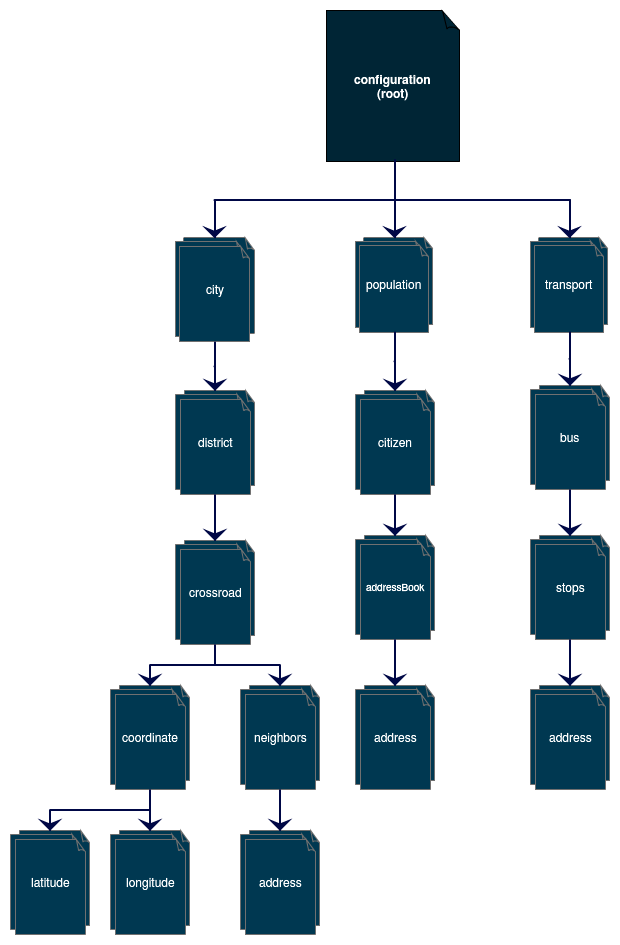
\includegraphics[scale=0.4]{images/configuration/XML-structure.png}
\caption{Struttura gerarchica del file XML}
\label{setup-configuration-xml-structure}
\end{figure}

\begin{itemize}
\item{\keyword{configuration}: è il nodo radice dell'intero documento;}
\item{\keyword{city}: esso definisce la struttura della città che si andrà ad implementare (può esserci un solo nodo città in tutto il documento); esso è composto dagli attributi:}
\begin{itemize}
\item{\keyword{name}: una stringa rappresentante il nome della città;}
\item{\keyword{hostname}: una stringa rappresentante l'indirizzo IP dell'\english{host} che eseguirà il nodo ``città'';}
\item{\keyword{port}: una stringa rappresentante la porta di rete in cui l'\english{host} ascolta richieste in ingresso.}
\end{itemize}
\item{\keyword{district}: esso definisce la struttura di uno dei distretti che compongono la città (possono essere presenti più nodi distretto); esso è composto dagli attributi:}
\begin{itemize}
\item{\keyword{name}: una stringa rappresentante il nome del distretto;}
\item{\keyword{hostname}: una stringa rappresentante l'indirizzo IP dell'\english{host} che eseguirà il nodo ``distretto'';}
\item{\keyword{port}: una stringa rappresentante la porta di rete in cui l'\english{host} ascolta richieste in ingresso.}
\end{itemize}
\item{\keyword{crossroad}: esso definisce la struttura di uno degli incroci che compongono la città (possono essere presenti più nodi incrocio); esso è composto dagli attributi:}
\begin{itemize}
\item{\keyword{name}: una stringa rappresentante il nome del distretto;}
\end{itemize}
\item{\keyword{coordinate}: contiene le coordinate geografiche dell'incrocio;}
\item{\keyword{latitude}: contiene la latitudine (espressa in px) dell'incrocio;}
\item{\keyword{longitude}: contiene la longitudine (espressa in px) dell'incrocio;}
\item{\keyword{neighbors}: contiene una lista di indirizzi che fanno rifermento ad incroci adiacenti;}
\item{\keyword{address}: specifica l'indirizzo di un incrocio nella struttura cittadina; esso è composto dai seguenti attributi:}
\begin{itemize}
\item{\keyword{ref}: una stringa con l'indirizzo di un incrocio.}
\item{\keyword{type}: una stringa che descrive il tipo di indirizzo, usato nella descrizione delle persone; (valori ammessi \english{home} - \english{work}).}
\end{itemize}
\item{\keyword{population}: esso definisce le persone che ``vivranno'' all'interno della struttura cittadina;}
\item{\keyword{citizen}: esso definisce una singola persona; esso è composto dagli attributi:}
\begin{itemize}
\item{\keyword{name}: una stringa contenente il nome della persona;}
\item{\keyword{vehicle}: una stringa contenente il veicolo utilizzato per spostarsi nella città (valori ammessi: \english{pawn} - \english{car} - \english{bus});}
\end{itemize}
\item{\keyword{addressBook}: contiene una lista di indirizzi che la persona visita durante la sua ``giornata tipo'':}
\item{\keyword{transport}: esso definisce i mezzi di trasporto pubblico che circolano nella città;}
\item{\keyword{bus}: esso definisce la struttura di un autobus; esso è composto dagli attributi:}
\begin{itemize}
\item{\keyword{run}: una stringa che permette di identificare l'autobus;}
\item{\keyword{capacity}: capacità di passeggeri che l'autobus può trasportare.}
\end{itemize}
\item{\keyword{stops}: una lista di indirizzi presso cui l'autobus effettua le fermate per permettere alle persone di salire/scendere.}
\end{itemize}

Si ricorda che tale file viene validato attraverso una grammatica ``XML Schema'' all'avvio del nodo ``città''. Qualora il file fornito in input non fosse conforme alle specifiche della grammatica il nodo bloccherà la sua fase di \english{bootstrap} non consentendo la prosecuzione. Tale scelta serve ad evitare a posteriori di avere errori di riferimenti dopo che la simulazione ha avuto il via.

\begin{lstlisting}[frame=single, caption={Esempio di configurazione tramite XML}]
<configuration>
 <city name="city" hostname="127.0.0.1" port="2552">
  <district name="city.d1" hostname="127.0.0.1" port="2553">
   <crossroad name="city.d1.c1">
    <coordinate>
     <latitude>25</latitude>
     <longitude>25</latitude>
    </coordinate>
    <neighbors>
     <address ref="city.d1.c2">
    </neighbors>
   </crossroad>
   <crossroad name="city.d1.c2">
    <coordinate>
    <latitude>125</latitude>
    <longitude>25</latitude>
    </coordinate>
    <neighbors>
     <address ref="city.d1.c1">
     <address ref="city.d2.c1">
    </neighbors>
   </crossroad>
  </district>
  <district name="city.d2" hostname="127.0.0.1" port="2554">
   <crossroad name="city.d2.c1">
    <coordinate>
     <latitude>225</latitude>
     <longitude>25</latitude>
    </coordinate>
    <neighbors>
     <address ref="city.d1.c2">
     <address ref="city.d2.c2">
    </neighbors>
   </crossroad>
   <crossroad name="city.d2.c2">
    <coordinate>
     <latitude>325</latitude>
     <longitude>25</latitude>
    </coordinate>
    <neighbors>
     <address ref="city.d2.c1">
    </neighbors>
   </crossroad>
  </district>
 </city>
 <population>
  <citizen name="Jacob" vehicle="pawn">
   <addressBook>
    <address ref="city.d1.c1" key="home" />
    <address ref="city.d2.c1" key="work"/>
   </addressBook>
  </citizen>
  <citizen name="Michael" vehicle="car">
   <addressBook>
    <address ref="city.d1.c2" key="home"/>
    <address ref="city.d2.c2" key="work"/>
   </addressBook>
  </citizen>
  <citizen name="Joshua" vehicle="car">
   <addressBook>
    <address ref="city.d1.c1" key="home"/>
    <address ref="city.d2.c2" key="work"/>
   </addressBook>
  </citizen>
 </population>
 <transport>
  <bus run="around_town" capacity="5">
   <stops>
    <address ref="city.d1.c1" />
    <address ref="city.d2.c1" />
    <address ref="city.d2.c2" />
    <address ref="city.d2.c1" />
   </stops>
  </bus>
 </transport>
</configuration>
\end{lstlisting}

\addcontentsline{toc}{section}{Esecuzione}
\section*{esecuzione}
\label{setup-execution}
Per l'esecuzione del simulatore è necessario possedere i due file eseguibili ottenuti tramite compilazione (nodo ``città'' e ``distretto'') ed il file XML che definisce la città. Oltre ai precedenti è necessario definire dei file testuali del tipo``chiave-valore'' contenenti informazioni identificative sulla tipologia di nodo che si intende istanziare; tali file sono necessari solamente per la fase di \english{debug} del progetto e si è progettato di eliminarli al completamento dell'intero progetto.

Tali file, uno per ogni nodo\footnote{Per il nodo ``città'' sono necessarie solamente le prime tre chiavi.} che si intende inizializzare, contengono le seguenti informazioni:

\begin{itemize}
\item{\keyword{city.name}: nome della città definito nel file XML;}
\item{\keyword{city.host}: indirizzo IP del nodo che esegue il nodo ``città'';}
\item{\keyword{city.port}: numero di porta in cui il nodo ``città'' rimane in attesa di connessioni entranti;}
\item{\keyword{district.name}: nome del distretto che il nodo andrà ad implementare;}
\item{\keyword{district.host}: indirizzo IP del nodo che esegue il nodo ``distretto'';}
\item{\keyword{district.port}: numero di porta in cui il nodo ``città'' rimane in attesa di connessioni entranti;}
\end{itemize}

\begin{lstlisting}[frame=single, caption={configurazioni per il nodo città}]
city.name=city
city.host=127.0.0.1
city.port=2552
\end{lstlisting}

\begin{lstlisting}[frame=single, caption={configurazioni per il nodo distretto d1}]
city.name=city
city.host=127.0.0.1
city.port=2552
district.name=city.d1
district.host=127.0.0.1
district.port=2553
\end{lstlisting}

\begin{lstlisting}[frame=single, caption={configurazioni per il nodo distretto d2}]
city.name=city
city.host=127.0.0.1
city.port=2552
district.name=city.d2
district.host=127.0.0.1
district.port=2553
\end{lstlisting}

Possedendo tutto il materiale necessario è ora possibile avviare il nodo città attraverso il seguente comando eseguito in una \english{shell}:

> \textbf{java -cp \$SCALA\_HOME/lib/scala-library.jar -jar city-assembly-1.0.jar city.txt city.xml}

In una diversa \english{shell} è possibile avviare un nodo distretto\footnote{I nodi ``distretto'' andranno avviati in seguito all'avvio del nodo ``città'' corrispondente} attraverso il seguente comando:

> \textbf{java -cp \$SCALA\_HOME/lib/scala-library.jar -jar district-assembly-1.0.jar d1.txt}

I precedenti comandi invocano la \ac{jvm} caricando, nel contesto di esecuzione, le librerie standard del linguaggio Scala; in seguito troviamo il percorso, nel \english{filesystem}, relativo a:

\begin{itemize}
\item{il \acs{jar} contenente l'eseguibile del nodo da istanziare;}
\item{il file identificativo del nodo.}
\end{itemize}

Si ricorda che essendo un prototipo di simulatore esso verrà eseguito per impostazione predefinita in \keyword{modalità di debug}, la quale consente la stampa a video dei vari comandi di \english{logging} presenti nel programma.